% ===== Opening: title, hook, the book, today's plan (~6 min) =====

% Title: the banner itself (common/art/title_banner.pdf, from banner/out/v2_glazz)
\begin{frame}[plain]
  \begin{tikzpicture}[remember picture, overlay]
    \node at (current page.center) {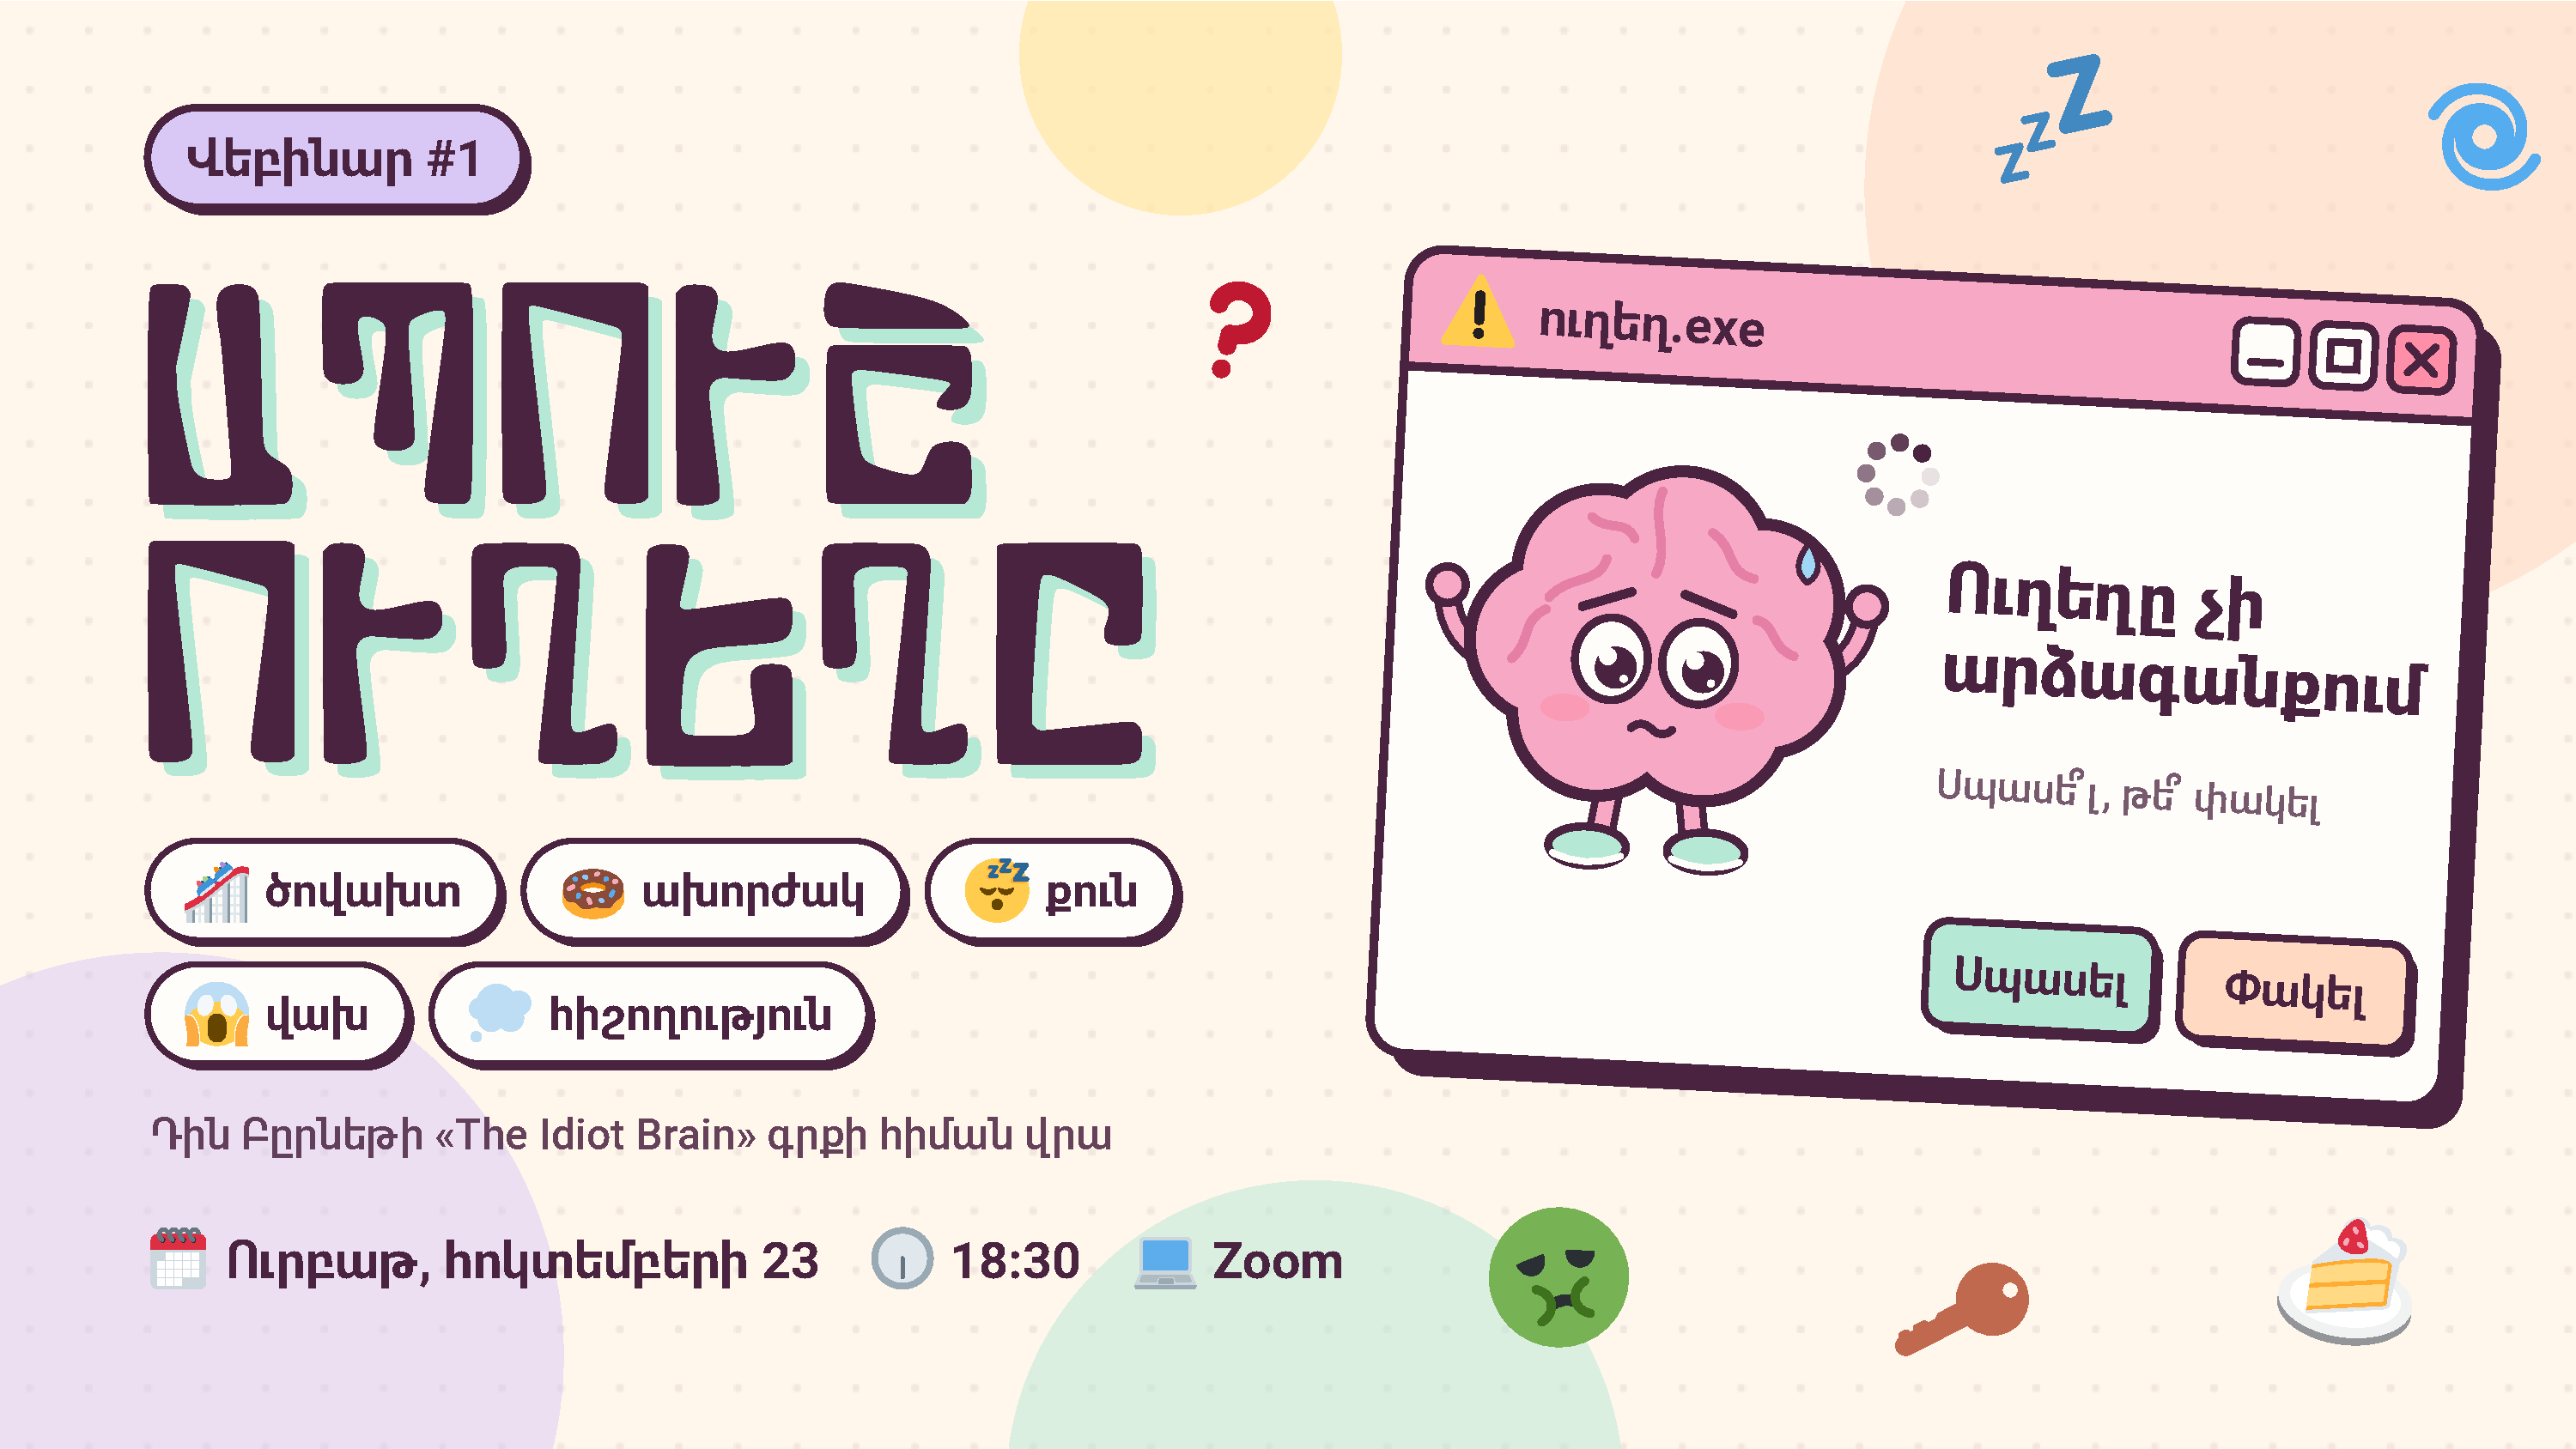
\includegraphics[width=\paperwidth]{title_banner.pdf}};
  \end{tikzpicture}
\end{frame}

% Hook: four everyday glitches; the audience types the ones they know
\begin{frame}{Ծանո՞թ է}
  \begin{columns}[c]
    \begin{column}{0.58\textwidth}
      \begin{popup}{ուղեղ.exe}
        {\blackfont\large Ուղեղը չի արձագանքում}\par\medskip
        \begin{enumerate}
          \item<2-> Մտար սենյակ ու մոռացար՝ ինչու
          \item<3-> Դեմքը ճանաչում ես, անունը՝ ոչ
          \item<4-> Կուշտ ես, բայց աղանդերի տեղ կա
          \item<5-> Քնելիս հանկարծ ցնցվում ես, կարծես ընկնում ես
        \end{enumerate}
      \end{popup}
    \end{column}
    \begin{column}{0.36\textwidth}
      \centering
      \mascot[3.2cm]{panic}\par\medskip
      \onslide<6->{%
      \begin{chatbox}
        Գրիր համարները, որոնք քեզ հետ եղել են (օր.՝ \textbf{1, 3})
      \end{chatbox}}
    \end{column}
  \end{columns}
\end{frame}

% The paradox of the whole series
\begin{frame}{Ամենաբարդ բանը, որ գիտենք}
  \begin{columns}[c]
    \begin{column}{0.46\textwidth}
      \begin{card}
        \centering
        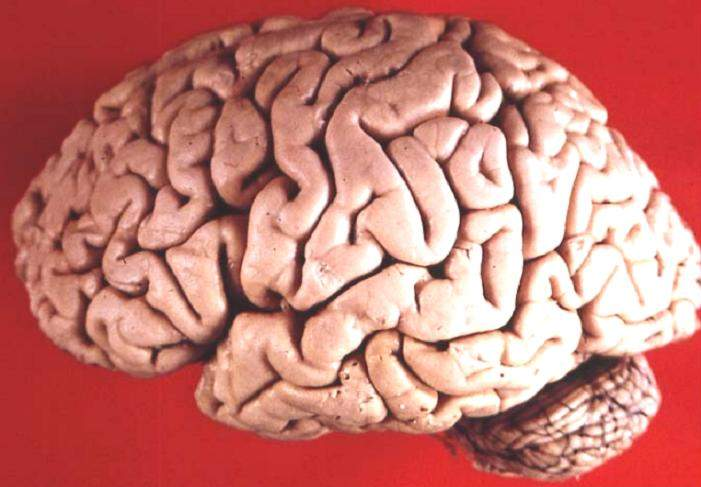
\includegraphics[width=0.85\linewidth]{brain_side.jpg}\par\smallskip
        {\blackfont\large Մոտ 86 միլիարդ նեյրոն}\par
        ու ավելի շատ կապեր (սինապսներ), քան աստղեր կան Ծիր Կաթինում
      \end{card}
    \end{column}
    \begin{column}{0.46\textwidth}
      \onslide<2->{%
      \begin{card}[colback=brainpink!30!cardwhite]
        \centering
        \mascot[2.4cm]{confused}\par\smallskip
        {\blackfont\large Եվ այդ նույն ուղեղը}\par
        մոռանում է, թե ինչու ես մտել խոհանոց \emoji{door}
      \end{card}}
    \end{column}
  \end{columns}
  \source{նեյրոնների թիվ՝ Azevedo et al., 2009}
\end{frame}

% The book and the author
\begin{frame}{Գիրքը և հեղինակը}
  \begin{columns}[T]
    \begin{column}{0.52\textwidth}
      \begin{card}
        {\blackfont\Large The Idiot Brain} {\small (2016)}\par
        «Ապուշ ուղեղը. նեյրոգիտնականը բացատրում է, թե իրականում ինչով է զբաղված գլուխդ»\par\medskip
        \begin{itemize}
          \item \textbf{Դին Բըրնեթ}՝ նեյրոգիտնական, դասավանդում էր Քարդիֆի համալսարանում
          \item Guardian-ում վարում էր «Brain Flapping» բլոգը
          \item Ազատ ժամերին՝ ստենդափ \emoji{grin}
        \end{itemize}
      \end{card}
    \end{column}
    \begin{column}{0.42\textwidth}
      {\blackfont\small Գրքի 8 գլուխը}\par\smallskip
      \chip[butter]{star}{Ներածություն}\par\smallskip
      \chip[mint]{rollercoaster}{1. Մարմնի կառավարում}\par\smallskip
      \chip[lavender]{thought}{2. Հիշողություն}\par\smallskip
      {\color{plum!55!cream}\small
      3. Վախ \quad 4. Խելք \quad 5. Ընկալում\\
      6. Անհատականություն \quad 7. Ուրիշ մարդիկ\\
      8. Երբ ուղեղը «փչանում» է}\par\smallskip
      \begin{card}[colback=mint!35!cardwhite]
        Կատակով, բայց աղբյուրներով
      \end{card}
    \end{column}
  \end{columns}
\end{frame}

% Plan for today
\begin{frame}{Այսօր}
  \begin{columns}[T]
    \begin{column}{0.31\textwidth}
      \begin{card}[colback=butter!45!cream]
        {\blackfont Ներածություն}\par\smallskip
        Ինչու է նեյրոգիտնականը ուղեղն «ապուշ» անվանում
      \end{card}
    \end{column}
    \begin{column}{0.31\textwidth}
      \begin{card}[colback=mint!45!cream]
        {\blackfont Մաս 1. Մարմինը}\par\smallskip
        \chip{rollercoaster}{ծովախտ}\par\smallskip
        \chip{doughnut}{ախորժակ}\par\smallskip
        \chip{sleeping}{քուն}\par\smallskip
        \chip{scream}{վախ}
      \end{card}
    \end{column}
    \begin{column}{0.31\textwidth}
      \begin{card}[colback=lavender!45!cream]
        {\blackfont Մաս 2. Հիշողությունը}\par\smallskip
        \chip{door}{կարճ ու երկար}\par\smallskip
        \chip{eyes}{դեմքեր ու անուններ}\par\smallskip
        \chip{wine}{ալկոհոլ}\par\smallskip
        \chip{crown}{եսասեր հիշողություն}\par\smallskip
        \chip{magnifier}{երբ այն փչանում է}
      \end{card}
    \end{column}
  \end{columns}
  \vspace{1mm}
  \centering
  {\small \emoji{coffee}\ Մեջտեղում՝ 5 րոպե ընդմիջում \quad \emoji{speech}\ Հարցերը գրեք չաթում ցանկացած պահի}
\end{frame}
